\section{Empirical Results}
\label{sec:bleuresult}

In this section, we present the empirical results to validate our hypothesis that 
\textit{BLEU is not effective in evaluating translation quality of source code migration task}
\subsection{Correlation between BLEU and Semantic scores}
To justify the first part of our hypothesis, BLEU score does not reflect well 
the semantic accuracy of results translated by a particular model, 
we show the relation between BLEU scores and human judgments via semantic scores. 
We use Pearson's correlation coefficient~\cite{PearsonCorrelation} to gauge
how strong their relation is. The correlation coefficient has value
between -1 and 1, where 1 indicates the strongest positive relation, -1
indicates the strongest negative relation, and 0 indicates no relation.

Figures~\ref{fig:BleuSemlpSMT} and~\ref{fig:BleuSemMppSMT} show the
scatter plots between two metrics: BLEU and Semantic. Each point
represents the scores of a pair of methods where its $x$-axis value is
for BLEU scores and $y$-axis value is for semantic scores. The
correlation coefficient between BLEU and semantic scores for the model
mppSMT is 0.523 and for the model lpSMT is 0.570. These possitive values 
are closer to 0.5 than to 1.0. This means there is a positive but weak 
relationship between BLEU score and semantic score. The weak correlations %help me to check grammar
between the metrics on the results translated by lpSMT and mppSMT are 
demonstrated in figures~\ref{fig:BleuSemlpSMT} and~\ref{fig:BleuSemMppSMT}.

%\emph{Observation 1:} 
In figure ~\ref{fig:BleuSemlpSMT}, for many specific values of BLEU, it 
is clear that associated semantic scores can be in a wide range. For 
instance, the BLEU score of 0.75, the associated semantic scores are 
from 0.25 to 1 \textbf{Ngoc: can u mark in the figure please}. Thus, from this 
observation, we conclude that the results migrated by certain models 
with high BLEU scores might not archive high semantic scores. 
%There are two reasons for this. 
%

In our sample set, these results can fall in two main cases. 
First, the translated methods might have multiple correct phrases, but in the 
incorrect order, those method can be incorrect, even incompliable.
%useless and justified as so in human judgment.
%
For example, in figure~\ref{fig:issueexample2}, the translated method
misplaces the position of the bracelet which makes the method has low
semantic score, but high BLEU score. 
%
%Another reason for this implication is that resulting method does not capture the important
%program elements. 
In other case, the migrated results are incomplete methods missing elements
that are trivial for the translation model, but this violate syntactic rules 
of the target language. For example, the result contains mostly keywords and
punctuation such as \code{if}, \code{public}, \code{()}, but misses
out the important program elements such as function calls or variable
names. In this case, it will have low semantic score while having
a moderate to high BLEU score. These circumstances indicate the weakness of BLEU metric 
in evaluating the translated results in programing language where syntaxes are well defined.

%\emph{Observation 2:} For a fixed value of Semantic score, there can
%be many associated BLEU values. Specifically, in the model lpSMT, with
%a Semantic Score of 1, the BLEU scores can vary greatly between 0-1,
%which is reflected on the top horizontal line of dots in the
%Figure~\ref{fig:BleuSemlpSMT}. Similarly, in
%Figure~\ref{fig:BleuSemMppSMT}, with the Semantic Score of 1, the BLEU
%scores are in the range of 0.5 to 1.
In the results translated by mppSMT (figure \ref{fig:BleuSemMppSMT}), 
for a particular value of  semantic score, there can be many associated 
BLEU values that spread out over a wide range. Specifically, 
with the absolute semantic score, the BLEU scores can vary greatly 
from 0.5 to 1.0. By this empirical results, it can be concluded that for 
some models, the method achieving higher semantic score does not necessarily 
have higher BLEU score. 

%From this observation, it can be implied that translated code can have
%low BLEU score, but high Semantic score. This can be explained by two
%reasons. 
From our sample data, we observe that there are two main reasons leading 
to this phenomenon.
%
First, a translated method can use different code structure from the 
reference one to perform the same functionality. Figure \ref{?} shows an example
that got maximum semantic score, but has low BLEU score, 0.4. In this example, 
the translated method uses a \code{for} loop instead of a \code{foreach} 
loop as in the reference code. The second reason causing this phenomenon 
is that the whitespace issue. For example, in figure \ref{?}, the translated method has the 
tokens \code{changeMe()}, but the reference method has \code{changeMe ()}. The former 
is interpreted as one token while the former is interpreted as two tokens. 
This situation reduces the precision on phrases, but the human subject still
evaluated the result with high semantic score. By this experiment, we also empirically 
verify the argument that the forcusing on the lexical precision of BLEU makes
this metric is not able to capture other aspects such as dependencies 
that contribute to the sementics of source code. This might lead to the ineffectiveness
of BLEU in reflecting the semantic accuracy of translated results. 

%TODO need to verify
In conclusion, BLEU does not reflect well the
semantics of source code, and it is not suitable to use in evaluating
semantic accuracy of a SMT-based code migration system.

\subsection{The Use of BLEU in Comparing Models}
To validate the use of BLEU in comparing different SMT-based code migration systems, we conduct study to see if an improvement in BLEU score over cross models reflects the improvement in translation quality represented by human judgments of semantic score between those models. For a same set of 375 original Java methods, the two models GNMT and mppSMT generates two sets of 375 translated methods. Each set has its own BLEU scores and Semantic scores.
We prove that an improvement in BLEU score does not sufficient nor necessary lead to an improvement in semantic score by showing:

1. From the sample, we choose pairs of results such that their GNMT's BLEU scores are higher than mppSMT's BLEU scores. Then, we perform t-test with alpha confident level of 0.95 on that subset to see if their GNMT's semantic scores are also higher or not. The results show a t-value of ... It meant we would reject the null hypothesis that GNMT's semantic scores are higher than mppSMT's ones. So, it can be concluded that an improvement in BLEU score is not sufficient to achieve a higher semantic score. 

2.  From the sample, we choose pairs of results such that their mppSMT's semantic scores are higher than GNMT's semantic scores. Then, we perform t-test with alpha confident level of 0.95 on that subset to see if their mppSMT's BLEU scores are also higher or not. The results show a t-value of ... It meant we would reject the null hypothesis that mppSMT's BLEU scores are higher than GNMT's ones. So, it can be concluded that an improvement in BLEU score is not necessary to achieve a higher semantic score. 

%We ignored pairs of translated results if they have the same BLEU score or Semantic score (136 of the cases). For the remaining results, we found out that in \textbf{34\%} of the cases, the change in BLEU score contradicts the change in Semantic score. It means an improvement in BLEU score leads to a decrease in Semantic score and vice versa. In other words, if one function is translated by two migration models, one-third of the time, the result which has higher BLEU score actually has lower translation quality than the other. 
Because of the results above, BLEU is not reliable to use in comparing different SMT-based migration models. 

\begin{figure}
\caption{BLEU metric vs Semantic metric (lpSMT model)}
\centering
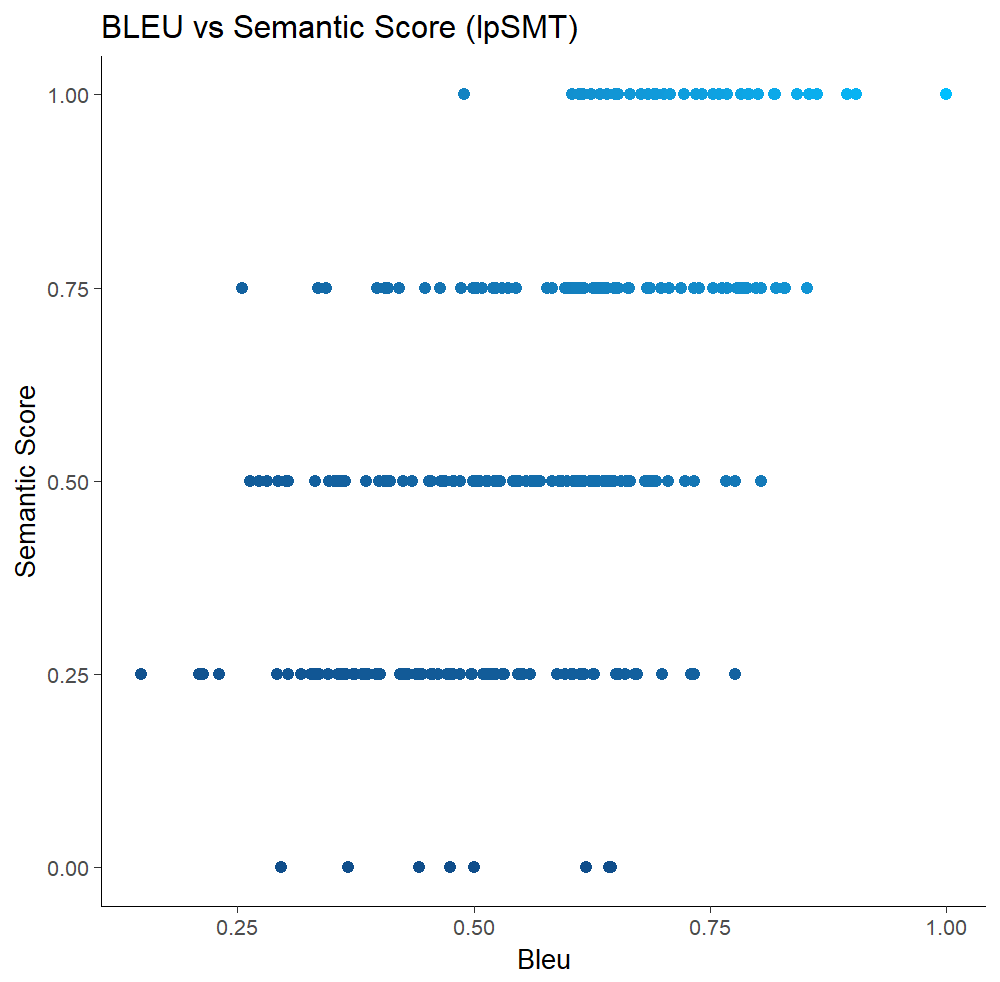
\includegraphics{img/bleuvssemantic_lpSMT.png}
\label{fig:BleuSemlpSMT}
\end{figure}

\begin{figure}
\caption{BLEU metric vs Semantic metric (mppSMT model)}
\centering
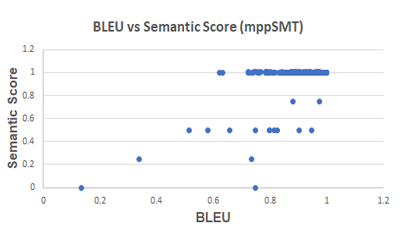
\includegraphics{img/bleuvssemantic_mppSMT.png}
\label{fig:BleuSemMppSMT}
\end{figure}

